%!TEX root = ../../../thesis.tex
\chapter{NEFI}

	Networks are amongst the central building blocks of many systems. Given a graph of a network, methods from graph theory enable a precise investigation of its properties. Software for the analysis of graphs is widely available and has been applied to study various types of networks. In some applications, graph acquisition is relatively simple. However, for many networks data collection relies on images where graph extraction requires domain-specific solutions.	In this chapter we introduce \NEFI, a tool that extracts graphs from images of networks originating in various domains. \NEFI provides a novel platform allowing practitioners to easily extract graphs from images by combining basic tools from image processing, computer vision and graph theory. Thus this novel software constitutes an alternative to tedious manual graph extraction and special purpose tools. In the context of this thesis \NEFI is used to extract graphs that represent vein networks formed by \P depicted in images acquired in the wet lab experiments discussed in the next chapter.

	As a large software project, \NEFI was created with the support of several individuals. We like to acknowledge Dr.~Adrian~Neumann who actively participated in this project from the start. Furthermore we like to thank Mag.~T.~Kehl and several students from Saarland University for contributing to the success of this project. A full list of acknowledgments is available at \NEFIs project page here: \href{http://nefi.mpi-inf.mpg.de}{http://nefi.mpi-inf.mpg.de}.



\section{Introduction}

	The study of complex network-like objects is of increasing importance for multiple scientific domains. 
	The mathematical study of networks, Graph Theory, formalizes a network's structure by modeling the constituents of a network as \emph{vertices} and the pairwise relations between them as \emph{edges}. Some communities traditionally refer to vertices as nodes or sites and to edges as arcs or links. Networks are ubiquitous in everyday life. Examples are as diverse as the Internet, social networks, transportation networks, metabolic networks, blood vessels or the vein networks of leaves. For a comprehensive review see~\cite{newman2003}. 

	In situations where the extraction of a mathematical graph from a physical network is easy, the size of graphs that can be analyzed may quickly increase from hundreds to millions of vertices. In such cases it is feasible to build large databases of networks which can be explored automatically using software relying on methods from statistics and graph theory. The combination of a large number of available graphs with dedicated methods of analyzing them yielded many results that changed our understanding of large scale network structures. Unfortunately, digitization of networks is not always easy and remains difficult for many types of networks. Examples include \eg leaf venations, blood vessels or food webs, and therefore ready-to-analyze datasets are often not available. In these cases, investigation on a larger scale requires tedious and sometimes error prone data acquisition.

	In many experimental settings networks are initially available as high quality images obtained under laboratory control. Before any analysis can take place, it is necessary to extract the associated graphs from these images. This requires the identification of vertices and edges within the depicted structure. This process can quickly become very work-intensive even for smaller networks, which makes automated solutions indispensable. 

	Leveraging advances in computer vision, several authors have proposed and successfully implemented solutions for domain specific graph extraction applications. The authors of~\cite{obara2012bioimage,obara2012contrast} consider the mycelial networks of \emph{P.~impudicus}, a member of the fungi. They use watershed segmentation in combination with a novel enhancement step designed to highlight curvilinear features in the input networks. Based on the segmented image a skeleton is computed and used to extract the graph representing the input network. The resulting method is designed to be brightness and contrast invariant in order to correctly extract the networks grown by \emph{P.~impudicus} from challenging noisy or low contrast images.
	
	Baumgarten et~al.~\cite{baumgarten2010detection,baumgarten2012computational} investigate the vein networks of \P using image processing techniques. For segmenting the input image they rely on careful constant thresholding followed by a sequence of restoration algorithms designed to remove artifacts introduced during thresholding. Next, the restored segmented image is used to compute a skeleton. After applying another sequence of correction steps, the skeleton is scanned to extract the graph of the input network.
 
	In \cite{chai2013recovering} a more general algorithm applicable to a variety of problems is proposed. Based on an original stochastic model, the authors use Monte Carlo sampling to obtain junction-points in the input image. This technically involved solution guarantees structural coherence for the resulting graph representation. Further examples include the extraction of road networks~\cite{nglt2006}, retinal blood vessel analysis~\cite{krause2013fast} and the extraction of plane graphs~\cite{hewrw2010}.

	The three above mentioned algorithmic solutions for the network extraction problem exhibit one or more of the following	limitations: 

	\begin{itemize}
		\item They do not build on top of well-established computer vision methods and tend to rely on ad-hoc algorithms. As a result the quality of the method and its implementation could likely be improved. In addition, a lot of time is spent on reimplementing algorithms that are already available in commong libraries. 

		\item They are not implemented at all or only available as pseudo-code.

		\item They are implemented but it is clear that the authors never intended anyone else to use their code. Implementations tend to neglect easy of use, distribution or issues of extendability.
	\end{itemize}

	One needs to remember that the primary objective of the work cited above is not the production of reusable software, but of algorithms and tools for solving a concrete research question at hand. The aim is to get the job done. As a result, the time for researching computer vision libraries and implementations, following best software engineering practice or writing documentation respectively is limited. 

	From experience we know that when trying to produce an easy-to-use software, a large part of the required work consists of specifying and improving the user-interface as well as working out minor bugs and annoyances. This type of work, while very time consuming, is essential for any software aiming to reach a non-negligible audience. However, efforts like these are hardly attractive to researchers whose focus is on obtaining the next result. While we understand that under these circumstances the aforementioned limitations arise naturally, we strongly believe that it is necessary to overcome those limitations in order to increase the value and the impact of scientific software in general and network extraction software in particular. It is possible to do better.

	To this end, we introduce \NEFI, a lightweight piece of ready-to-go software intended to enable the non-expert to automatically extract networks from images. \NEFI constitutes an extensible framework of interchangeable algorithms accessible through an intuitive graphical user interface. 

	We emphasize at this point that we do not claim to introduce novel techniques for image processing or computer vision. Instead, our contribution consists of a reusable, flexible and easily extendable toolbox combining well-known methods, which have become standard in their respective fields of origin, in a meaningful way. By introducing \NEFI, we hope to make these methods more widely accessible, especially to practitioners that are unfamiliar with them.

	\NEFIs segmentation is based on a combination of standard routines available in~\href{http://opencv.org/}{OpenCV},~(2015),~\cite{opencv}. These algorithms are known to perform well on clean and uncluttered images obtained under controlled laboratory conditions. However, on more challenging inputs of low contrast, strong gradients or similar irregularities, their performance is severely reduced. Nevertheless, in these cases more involved algorithms, currently not implemented as part of a reliable library and thus not integrated into \NEFI, may still be able to process these images. To help meet this situation, \NEFI was designed with extendability in mind. As a result users will find it easy to build on-top of \NEFIs code in order to add their own implementations of more sophisticated methods. 

\section{Network Extraction From Images}	%	2298 words

	NEFI features a collection of image processing routines, segmentation methods and graph algorithms designed to process 2D digital images of various networks and network-like structures. Its main function is executing a so-called extraction pipeline, designed to analyze the structures depicted in the input image. An extraction pipeline, for short pipeline, denotes an ordered sequence of algorithms. A successful execution will return a representation of the network in terms of an edge-weighted undirected planar graph. Computed weights include edge lengths and edge widths. Once the graph is obtained, available graph analysis software~\cite{ICWSM09154,snap,batagelj1998pajek,5437689,loscalzo2008social,hagberg2008exploring} or custom written scripts can be deployed to investigate its properties.

	A typical pipeline combines algorithms from up to four different classes: preprocessing, segmentation, graph detection and graph filtering, see \Fref{fig:workflow}. A more detailed description follows below. 
	
	\begin{figure}
		\centering
		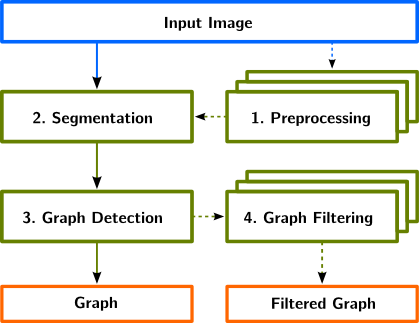
\includegraphics[width=\oneimagewide,keepaspectratio]{workflow.png}
		\caption[Pipeline components of \NEFI]{A flow chart illustrating \NEFIs pipeline components in green boxes. Dashed arrows depict optional sections of the pipeline. Blue and orange boxes denote \NEFIs input and possible outputs respectively.}
		\label{fig:workflow}
	\end{figure}

	For each pipeline section, \NEFI typically offers several interchangeable algorithms to choose from. After executing preprocessing routines, a segmentation algorithm separates foreground from background. Then the foreground is thinned to a skeleton from which the vertices and edges of the graph are determined. In the process various edge weights are computed. Finally, the graph can be subjected to a variety of useful graph filters. \Fref{fig:pipeline} illustrates the intermediate results of \NEFIs pipeline steps listed in the order of their execution. When a pipeline is executed, \NEFI makes all intermediate results available via its clean and intuitive GUI, see \Fref{fig:nefi_gui}. 

	\begin{figure}
		\centering
		\subfloat[\NEFIs pipeline - Input image][Input image.]{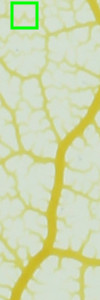
\includegraphics[width=0.15\linewidth,keepaspectratio]{pipeline/input.jpg}\label{fig:pipeline:input}}\quad
		\subfloat[\NEFIs pipeline - Segmented image][Segmented image.]{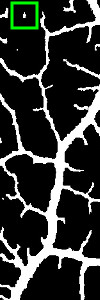
\includegraphics[width=0.15\linewidth,keepaspectratio]{pipeline/segmented.jpg}\label{fig:pipeline:segmented}}\quad
		\subfloat[\NEFIs pipeline - Skeletonized image][Skeletonized image.]{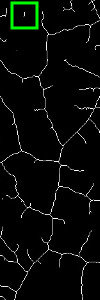
\includegraphics[width=0.15\linewidth,keepaspectratio]{pipeline/skeleton.jpg}\label{fig:pipeline:skeleton}}\quad
		\subfloat[\NEFIs pipeline - Detected graph][Detected graph drawn ontop of the input.]{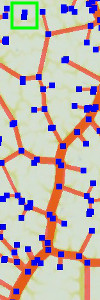
\includegraphics[width=0.15\linewidth,keepaspectratio]{pipeline/full_graph.jpg}\label{fig:pipeline:full_graph}}\quad
		\subfloat[\NEFIs pipeline - Filtered graph][Filtered graph drawn ontop of the input.]{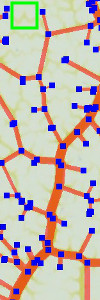
\includegraphics[width=0.15\linewidth,keepaspectratio]{pipeline/largest_component.jpg}\label{fig:pipeline:largest_component}}\quad
		\caption[\NEFIs pipeline executed]{Direct comparison of \NEFIs pipeline steps given a slice of an image of a slime mold (\P). From left to right: input image, segmented image, skeletonized image, detected graph and filtered graph. The green square contains a very faint vein which the segmentation did not pick up fully. Thus, the skeleton becomes fragmented which leads to spurious vertices in the detected graph. By applying a graph filter we remove stray vertices without manipulation of the segmented or the skeletonized image. Similar filtering can remove ``dead-ends'', \ie vertices that do not belong to any cycle in the graph.}
		\label{fig:pipeline}
	\end{figure}

	Using the GUI all basic functions of \NEFI can be accessed in an intuitive fashion. To facilitate ease-of-use, most of \NEFIs algorithms come with default parameters based on the settings in \href{http://opencv.org/}{OpenCV}~\cite{opencv}, which were found to perform well on our test sets as well as on many other images.

	\begin{figure}
		\centering
		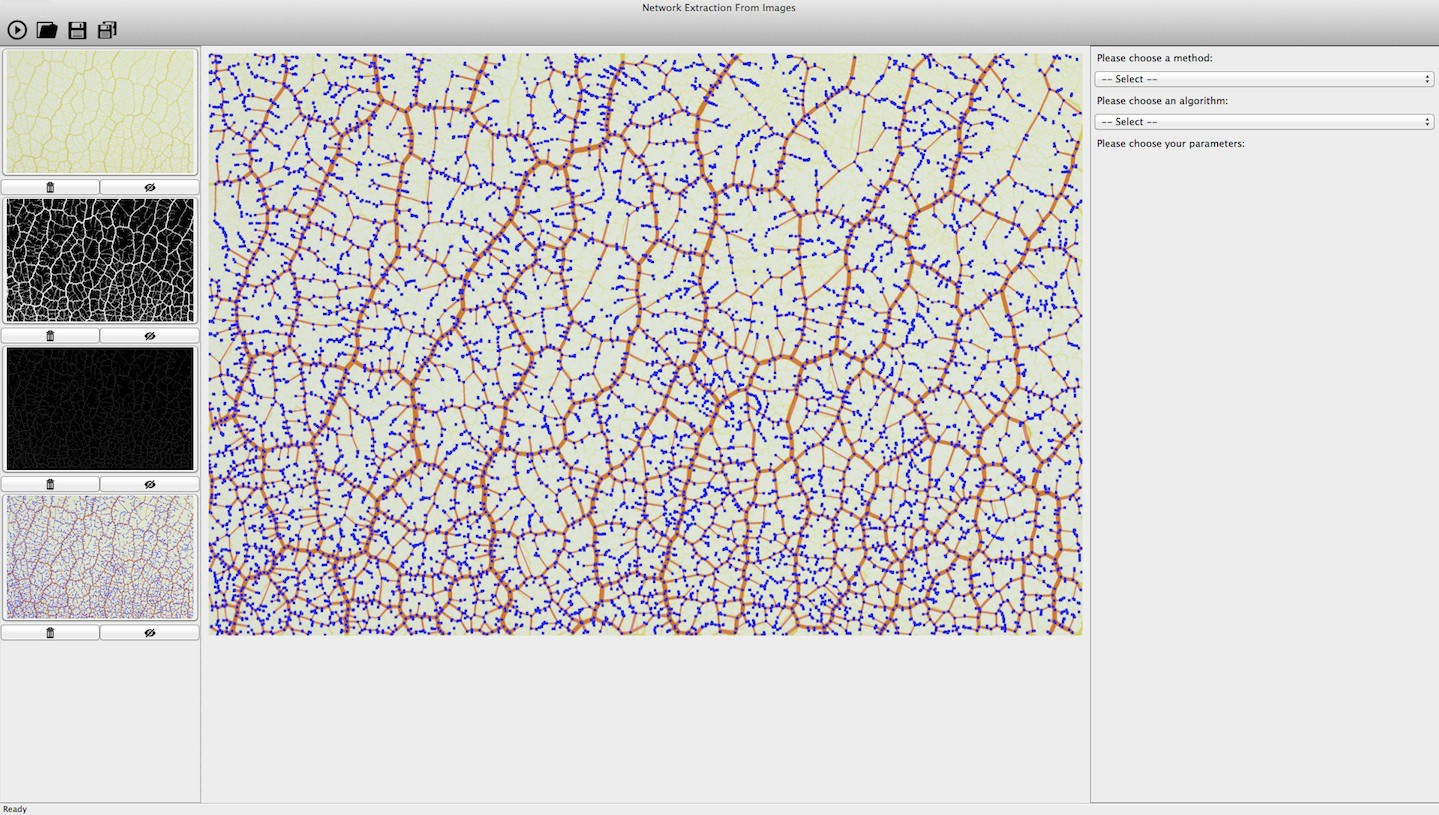
\includegraphics[width=\oneimagewide,keepaspectratio]{gui.jpeg}
		\caption[\NEFIs graphical user interface.]{A screenshot of \NEFIs GUI running on Mac OS. On the left hand side \NEFI lists intermediate results as thumbnails. Bringing the final result to the center workspace allows for direct visual assessment of the quality of the extracted graph. On the right hand side \NEFIs pipeline elements can be accessed via drop-down menus. The image was produced in a collaboration with the KIST Europe.}
		\label{fig:nefi_gui}
	\end{figure}

	There are various predefined pipelines to get started immediately. Alternatively, users may freely combine the various methods to build custom pipelines. Both approaches allow the user to experiment with the available methods in order to close in on the optimal settings for the data at hand. Once a pipeline is constructed, it can be saved and reused. \NEFIs simple pipeline concept together with a self-explanatory graphical user interface make working with \NEFI intuitive and straightforward. \NEFI also offers a command-line mode, which is suited for batch processing large quantities of input images.

	NEFI comes with a number of example images from different domains which we use to produce the figures in this work. \Fref{fig:physarum} and \Fref{fig:dragonlfy} show \NEFIs output on two images using predefined pipelines. Blue squares denote the vertices and red lines the edges of the detected graph. The thickness of the detected edges corresponds to thickness of the depicted structures. For comparison the extracted graph is drawn on top of the input image. We present a detailed quantitative evaluation in a later section.


	\begin{figure}
		\centering
		\subfloat[\P: Input to \NEFI][]{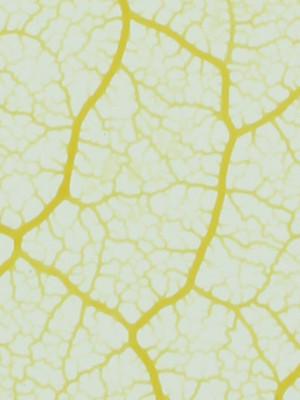
\includegraphics[width=\twoimageswide,keepaspectratio]{p_polycephalum.jpg}\label{fig:physarum:input}}
		\subfloat[\P: Output of \NEFI][]{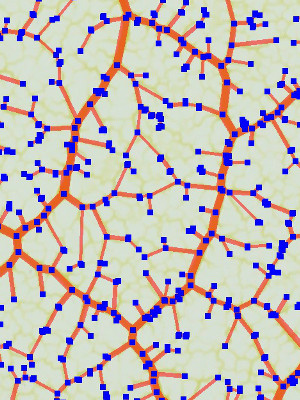
\includegraphics[width=\twoimageswide,keepaspectratio]{p_polycephalum_graph.jpg}\label{fig:physarum:graph}}
		\caption[\P: Input and output of \NEFI]{Extracted graph of the network formed by \P. The left hand side shows the input image depicting the network. The right hand side shows the extracted graph overlayed on top off the same image for direct comparison. Note, that no filters have been applied. The image was produced in a collaboration with the KIST Europe.}
		\label{fig:physarum}
	\end{figure}

	\begin{figure}
	\centering
		\begin{tikzpicture}
			\begin{scope}[spy using outlines={rectangle,black,magnification=2.5,size=4cm}]
			\node {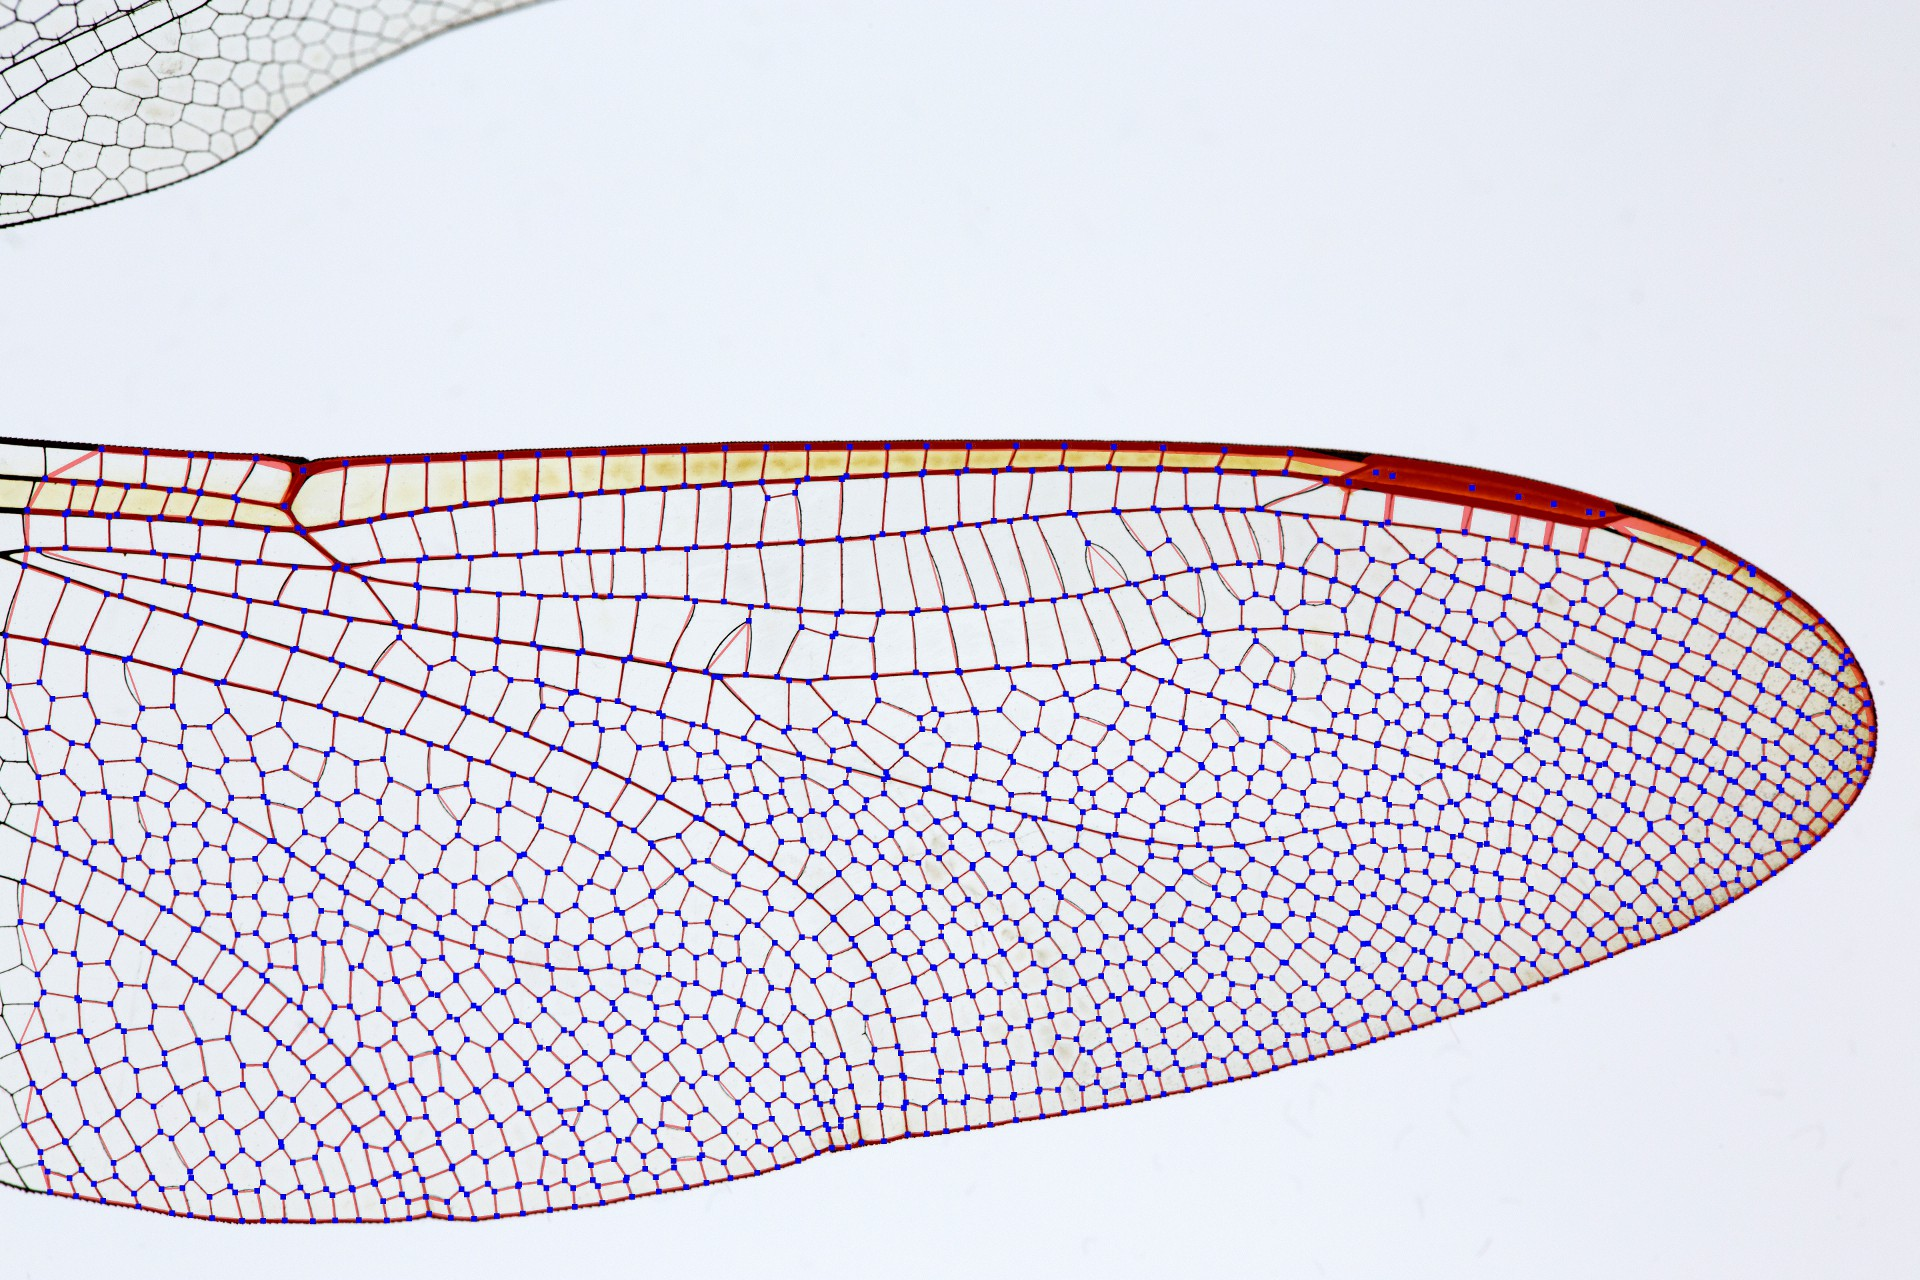
\includegraphics[width=\oneimagewide,keepaspectratio]{dragonfly_optimal.jpeg}};
			\spy on (-1,-1) in node (a) [left] at (5.5,-1.5);
			\end{scope}
		\end{tikzpicture}
	\caption[\A: Output of \NEFI]{Extracted graph of the vein network exhibited by a wing of a dragonfly (\A). Note, that after the use of various filters a very clean-looking graph is obtained. Image courtesy of Pam and Richard Winegar.}
	\label{fig:dragonlfy}
	\end{figure}


	We stress that \NEFI can deal with a range of inputs from various domains as long as they are of sufficient quality. In addition to the examples shown above, it has been successfully used to process images of natural (\eg leaf venation, patterns of mud cracks) as well as man-made structures (\eg tilings). It is also straightforward to add custom extensions. We provide a well documented platform which allows programmers to include more specialized segmentation algorithms or additional graph filters. For an overview of alternative graph extraction approaches see for example~\cite{dehkordi2011review}.

	Next, we discuss the purpose and design of each major stage of the pipeline and highlight some of \NEFIs strong points.


	\subsection{Preprocessing Collection}

		The preprocessing section of the pipeline offers various standard image processing algorithms intended to be used prior to the segmentation step. Preprocessing methods may be exploited to positively affect the output of the segmentation step. For example, adding a slight blur to an input image may benefit the overall result by reducing the amount of spurious white pixels appearing in the segmented image. However, blurring too much will remove detail and reduce accuracy in determining the thickness of depicted edges. As a result, we recommend to experiment with different approaches and parameter settings in order to decide how to use preprocessing. For images of sufficient quality we found that excellent results can be obtained without preprocessing. 

		NEFI relies on \href{http://opencv.org/}{OpenCV}~\cite{opencv} for preprocessing and offers Gaussian and Median Blurring, Denoising as well as Bilateral Filtering.

	\subsection{Segmentation Collection}

		The goal of the segmentation step is separating the image foreground, \ie the structures of interest, from the remaining image. \NEFI builds on top of \href{http://opencv.org/}{OpenCV}~\cite{opencv} combining different segmentation algorithms. The general-purpose algorithms shipped with \NEFI have become standard in image processing and perform reliably well if input images are clean, devoid of strong gradients and have a good contrast between fore- and background. Conversely, if the input becomes more challenging, the effectiveness of \NEFIs segmentation degrades quickly and more complex or domain-specific algorithms become necessary. We defer a quantitative study of how the properties of the input image affect \NEFIs performance to the Section \emph{Evaluation}. 

		\NEFIs segmentation is designed such that several algorithms can be used interchangeably. We included basic thresholding algorithms like Otsu's method~\cite{otsu1979} or adaptive thresholding as well as more involved segmentation routines such as guided watershed~\cite{watershed91} and the GrabCut algorithm~\cite{grabcut2004}. The last two methods receive as an additional input a so-called marker. The better the markers approximate the foreground, the better these algorithms work. \NEFI offers several marker strategies which can be used interchangeably together with the respective marker based segmentation routines. 

		Interchangeability of the algorithms is a core design principle of all pipeline steps.

		This design facilitates easy experimentation with different methods. Our own experience shows that often it is not clear a priori which method will work best for a given input image. A sensitive method may yield excellent segmented images and very detailed graphs, however its sensitivity increases the chance false positives nodes and edges. Since the ideal ideal choice usually depends on several competing factors, easy experimentation with different settings coupled with immediate visual feedback from the GUI become major strong points of \NEFI.

		Flexibility is not limited to the algorithms that come with \NEFI. Modular software design makes it easy to integrate additional methods and access them via the GUI. It is likely that sooner or later input images will be encountered in practice that are too challenging for the core algorithms available in \NEFI to deal with. In these cases a potential user may choose to implement additional, perhaps domain-specific, methods capable of meeting the challenge at hand. When extending \NEFI, the user can build on existing modules, yielding more reliable code which is easier to understand and maintain. In this way \NEFI is set up to support future development and growth.

	\subsection{Graph Detection Collection} 

		The graph detection collection consists of algorithms that take a segmented image as input and determine the nodes and the edges of the output graph. We offer a colloquial description of the actual algorithm because we do not rely on well-documented library code for this section of the pipeline. 

		The first step for graph detection is called thinning. Here we reduce the segmented foreground such that every line is only one pixel thick, while preserving the connectivity properties of both the foreground and the background pixels. The result of this process is called the skeleton of the segmented image. To do so we implemented the algorithm by Guo and Hall~\cite{guo1989parallel}. It always produces thin results and preserves 8-connectivity of the foreground pixels. The latter is essential for preventing all sorts of erroneous edges and spurious nodes. For this reason we choose Guo-Hall thinning over other available thinning algorithms. A pure Python implementation proved to be fairly slow, hence we chose to implement this function as a C extension. 

		For fairly thin and network-like foreground structures this method is nearly flawless and finds a skeleton where the lines lie in the center of the foreground areas. However, large foreground structures that do not resemble networks lead to artifacts in the skeleton whose exact shape depends on the noise present at their borders.

		Once the skeleton is established, we use it to detect the positions of nodes. For this purpose we adapt criteria from a thinning algorithm by Zhang and Suen~\cite{zhang1984fast}. A white skeleton pixel becomes a node in the output graph if its removal creates exactly one or at least three 4-connected white components in its 1-neighborhood. In the former case the pixel forms the end of a path, \ie a node of degree $1$, in the latter case is the meeting point of at least three edges, \ie a node of degree $\ge 3$.

		Note that due to this step, the maximum degree of the graphs we detect is limited to four. This is inevitable if nodes are detected at single-pixel locations. For higher degree nodes we will create several nodes of smaller degree that are very close to each other. In this way it is possible to establish the correct large node degree by merging the smaller degree nodes in a later post-processing step.

		Given the node positions, it is very simple to find the edges by establishing the paths of pixels between them. We perform a variant of breadth first search on the white pixels in the skeleton, starting from each node simultaneously. Each white pixel around a node gets a unique number and a queue. In each step we iterate over all queues and take out the first pixel. If it is unmarked, we mark it with the unique number of this queue and enqueue all its white neighbors. Otherwise, we have detected an edge, \ie there is a path along white pixels that connects two nodes.

		While walking along the pixels we record the length of the edge in units of pixel. Horizontal and vertical steps count as one unit, diagonal steps count as $\sqrt 2\approx 1.41$ units.

		The diameter of an edge is calculated by computing the distance transform of the segmented image. Next, we assume that the path of skeleton pixels representing an edge approximately goes through the middle of the real edge seen in the input image. Under this assumption, which we found to be approximately true for our test images, computing the diameters becomes a simple lookup of each edge-pixel from the skeleton in the distance transformed image. Since doing so we obtain the diameter for every pixel belonging to an edge, we can easily compute statistical quantities over the diameter values.

		For handling the graph in terms of data-structures, we rely on \href{https://networkx.github.io/documentation/latest/index.html}{NetworkX}~\cite{networkx}.

	\subsection{Graph Filter Collection}

		The graph filter collection offers the possibility to add powerful processing steps that directly apply to the graph obtained after graph detection. Unlike the methods in the preprocessing collection, graph filters do not affect segmentation and graph detection.

		Often it is possible to improve the quality of the obtained graph by removing unwanted artifacts caused by segmentation or later processing steps. A common strategy, used for example in \cite{baumgarten2010detection, baumgarten2012computational}, consists of ``reparing'' the errors present in the skeleton due to bad segmentation using heuristics or user assisted methods. While such methods can do well, they carry the potential risk of introducing additional errors. 

		\NEFI pursues a novel approach exploiting knowledge of the structure of the extracted graph together with dedicated filtering methods. We start by using very sensitive segmentation retaining a maximum of structural information. We do not manipulate the resulting segmented image or the skeleton at all. Based on the skeleton we establish the graph which in general will contain some artifacts. For example, if the network in the input image is large and connected, the resulting graph will consist of a large connected component plus a number of spurious smaller components caused by noise. Such components can easily be spotted when one compares the original images with the output graph. Using one of \NEFIs graph filters they can be removed effectively and safely, increasing the degree of similarity between the original network and the extracted graph. Since the effects of filtering the graph can immediately be evaluated by visual inspection, we prefer graph filtering over less transparent approaches aiming to improve the graph before it was established. \Fref{fig:pipeline} illustrates the use of filtering.

		We have used filtering with sensitive segmentation to obtain surprisingly good results. Overly sensitive segmentation picks up fine detail but is also prone to create artifacts due to noise. However, almost all of the artifacts result in very small components that can easily be removed by filtering. The desired detail will remain mostly unaffected because it is part of the largest component. The graph depicted in \Fref{fig:dragonlfy} was obtained using this technique.

		Filtering may also be used to remove parts of the graph which are not of interest. The following filters are predefined in \NEFI. A filter removing everything not in the largest connected component, one smoothing vertices of degree two except if this introduces parallel edges and finally, one which removes all vertices and edges that are not contained in a cycle. Filters may be freely combined in any order. Naturally, the filter collection is designed for extendability which means that users may add their own filters to the existing collection.

		Graph filtering and its various applications delivers excellent results. To our knowledge, no other software offers such flexible tools as part of its core workflow.

\section{Evaluation}

	To assess \NEFIs performance we quantify the quality of the resulting output graphs as a function of input images of varying difficulty. To this end we define a quality measure that captures the degree of similarity between the graphs computed by \NEFI and the networks depicted in the input. While to a certain degree said similarity can be determined for a small set of instances by visual inspection, a dedicated measure allows us to systematically and reproducibly investigate whether \NEFIs graph extraction is reliable. As an additional metric of interest, we report \NEFIs speed which becomes relevant as soon as one starts to process large batches of input images. 
 
	\subsection{Using a Graph Similarity Measure to Evaluate NEFI}

		Our quality measure needs to quantify the degree of congruence between the graph depicted in the original input image $i$ and the graph computed by \NEFI.  

		Let $A = (V_A, E_A)$ be the \emph{true} graph correctly describing the structure depicted in $i$, with $V_A$ and $E_A$ denoting its vertex and edge set respectively. We call $A$ the \emph{ground truth}, which is of course not known in general. Furthermore, let $B$ denote the graph obtained by executing one of \NEFIs pipelines. Note that, $A, B \in \mathcal{G}$, where $\mathcal{G}$ denotes the set of undirected edge-weighted planar graphs where vertices are labeled with their respective euclidean coordinates in the plane. With these definitions we propose a similarity measure $s$ mapping any pair of graphs $A,B \in \mathcal{G}$ onto a number $s \in [0,1]$. Then, this number $s$ serves as our similarity measure. 

		To obtain $s$, we compute a correspondence of vertices in $A$ to vertices in $B$. Two edges $e \in E_A$ and $f \in E_B$ then correspond if their endpoints correspond. We choose the correspondence such that the following intuitive notion of similarity are optimized.

		\begin{enumerate}
		\item Positions of vertices in $V_A$ are similar to positions of corresponding vertices in $V_B$.  
		\item Edges in $E_A$ including their weights are similar corresponding edges in $E_B$. 
		\end{enumerate}

		We require that the measure $s$ is maximal if any graph $A$ is compared with itself, that is $s(A,A) = 1$. Consequently, if $A$ is completely different from $B$ we have $s(A,B) = 0$. This minimum value is assumed if no viable correspondence between $V_A$ and $V_B$ can be found. Naturally, the value of $s(A,B)$ increases (decreases) if the similarity between $A$ and $B$ increases (decreases).

		An exact definition of $s$ and the notions of \emph{similarity} and \emph{correspondence} is given in the following section.

	\subsection{Definition of the Similarity Measure}

		In order to determine the overall quality of \NEFIs output we need to quantify the degree of similarity between two graphs $A = (V_A, E_A)$ and $B = (V_B, E_B)$ using a graph similarity measure. Let $A, B \in \mathcal{G}$, where $\mathcal{G}$ is a set of undirected edges-weighted planar graphs where the nodes are labeled with their respective coordinates in the eucledian plane. Then we may define a similarity measure $s$ as follows:
		
		\begin{gather}
		s : \mathcal{G} \times \mathcal{G} \mapsto [0,1] \notag \\
		s(A,B) = \text{matching}(A,B) \quad \quad \forall \ A, B \in \mathcal{G}
		\end{gather}

		Where $\text{matching}(A,B)$ denotes the normalized cost of a minimum cost graph matching problem which we will define shortly. Given this definition the degree of similarity between $A$ and $B$ is quantified by the value of $s(A,B)$. The similarity measure we propose has the following desirable properties:


		\begin{itemize}
			\item $A$ compared to itself yields a maximum similarity score of $s(A,A) = 1$.
			\item If there are no vertices in $V_A$ with corresponding similar nodes in $V_B$ and no edges $E_A$ with corresponding similar edges in $E_B$ the minimum similarity score of $s(A,B) = 0$ is obtained.
			\item The similarity score $s(A,B)$ increases (decreases) if the similarity between $A$ and $B$ increases (decreases).
		\end{itemize}

		We proceed with making the notions of \emph{similarity} and \emph{correspondence} more precise by constructing a minimum cost graph matching problem. Given the two graphs $A,B \in \mathcal{G}$, let $n_A,n_B$ denote the number of nodes and $m_A,m_B$ denote the number edges of the respective graphs. Note that $n_A$ and $n_B$ can differ, as can $m_A$ and $m_B$.

		We can now define a matching between $A$ and $B$ consisting of three parts. First we define a matching between the node sets $V_A, V_B$, then we define a matching between the edges sets $E_A, E_B$ and finally we introduce a coupling between the two. To obtain a solution to the final problem we rephrase the combined matching problem as an integer linear program and obtain a solution using IBM's CPLEX solver~\cite{cplex2009v12}. For ease of exposition, however, we discuss the problem using the language of matchings.

		For the node matching, we match each node $i \in V_A$ with at most one node $j \in V_B$. We define a variable $x_{ij}$ that is $1$ if we match $i$ with $j$ and $0$ otherwise. With a match we associate a cost of $\Delta_V(i,j)$. The function $\Delta_V(i,j)$ returns the euclidean distance between node $i$ and node $j$. If any node $u$ remains unmatched, we assign a penalty of $p_V(u)$ to it. A node can either be penalized or matched but not both. We thus compute a minimum cost node matching, in which it is favorable for a node $i \in V_A$ to find a match with a node $j \in V_B$ such that $i$ and $j$ are close in distance as measured by $\Delta_V(i,j)$. Two nodes are thus \emph{similar} if their euclidean positions are almost the same. For any given node in $V_A$ there can be potentially many similar nodes in $V_B$, all of which are candidates for a match. Amongst all candidates the minimum cost matching selects pairs that are most similar. We call such the selected pairs of similar nodes \emph{corresponding}.

		The edge matching proceeds analogously to the node matching. Each edge $e \in E_A$ is matched with at most one edge $f \in E_B$. We denote this match with a decision variable $y_{ef}$ and associate a cost of $\Delta_E(e,f)$ with it. The function $\Delta_E(e,f)$ returns the sum of the differences in edge weights between edge $e$ and edge $f$. If any edge $d$ remains unmatched, we assign a penalty of $p_E(d)$ to it. An edge can either be penalized or matched but not both. We thus compute a minimum cost edge matching, in which it is favorable for an edge $e \in E_A$ to find a match with an edge in $f \in E_B$ such that $e$ and $f$ are close in weights as measured by $\Delta_E(e,f)$. Two edges are thus \emph{similar} if their weights are almost the same. For any given edge in $E_A$ there can be potentially many similar edges in $E_B$, all of which are candidates for a match. Amongst all candidates the minimum cost matching selects pairs that are most similar. We call such a matching pair of edges \emph{corresponding}.

		As of yet both matchings are independent of each other. In particular this allows an edge $e \in E_A$ to be matched with an edge $f \in E_B$ independently from their respective positions in the plane as long as they have similar weights! A more meaningful matching favors pairing edges where the endpoints of both edges are also similar to each other. Hence, start and end nodes of corresponding edges should be pairwise corresponding themselves. In other words, head and tail nodes of both edges are geographically close respectively. 

		This additional constraint suggests a dependence between node and edge matching. To enforce it we add the constraint that an edge $e = (a,b) \in E_A$ can only be matched to an edge $f = (a',b')$ if the respective nodes are pairwise matched as well. That is, we require $a$ to be matched to $a'$ and $b$ to be matched to $b'$ or alternatively $a$ to be matched to $b'$ and $b$ to be matched to $a'$. 

		By combining node matching, edge matching and the additional coupling constraint we obtain the final minimum cost matching problem. We rephrase the uncoupled matching problem as an integer linear program (ILP) as follows:

		\begin{alignat}{4}
		\textbf{Minimize:} &  & \ \ f = &\sum_{ \substack{i \in V_A \\ j \in V_B }} \Delta_V(i,j) x_{ij}  &+  \sum_{ \substack{i \in V_A}} p_{V}(i) \overline{x}_{i} &+   \sum_{ \substack{j \in V_B}} p_{V}(j) \overline{x}_{j} & + \notag \\ 
		 &   & \ \     &\sum_{ \substack{e \in E_A \\ f \in E_B }} \Delta_E(e,f) y_{ef}  &+  \sum_{ \substack{e \in E_A}} p_{E}(e) \overline{y}_{e} &+   \sum_{ \substack{f \in E_B}} p_{E}(f) \overline{y}_{f} &
		\end{alignat}

		% \begin{align}
		% \textbf{s.t.:} 	&&x_{ij} \in \{0,1\} &&i \in V_A &&j \in V_B \\
		% 				&&y_{ef} \in \{0,1\} &&e \in E_A &&f \in E_B \\
		% 				& &\forall \ i \sum_{j} x_{ij} \leq 1  &&\forall \ j \sum_{i} x_{ij} \leq 1 \\
		% 				& &\forall \ e \sum_{f} y_{ef} \leq 1  &&\forall \ f \sum_{e} y_{ef} \leq 1 \\
		% 				& &\overline{x}_{i} =  1 - \sum_{j \in V_B} x_{ij} &&\overline{x}_{j} =  1 - \sum_{i \in V_A} x_{ij} \\          
		% 				& &\overline{y}_{e} =  1 - \sum_{f \in E_B} y_{ef} &&\overline{y}_{f} =  1 - \sum_{e \in E_A} y_{ef}                                        
		% \end{align}

		\begin{align}
		\textbf{s.t.:} 	&&x_{ij} \in \{0,1\} &&i \in V_A &&j \in V_B \\
						&&y_{ef} \in \{0,1\} &&e \in E_A &&f \in E_B                                    
		\end{align}

		\begin{align}
		\textbf{s.t.:} 	& &\forall \ i \sum_{j} x_{ij} \leq 1  &&\forall \ j \sum_{i} x_{ij} \leq 1 \\
						& &\forall \ e \sum_{f} y_{ef} \leq 1  &&\forall \ f \sum_{e} y_{ef} \leq 1				                               
		\end{align}

		\begin{align}
		\textbf{s.t.:} 	& &\overline{x}_{i} =  1 - \sum_{j \in V_B} x_{ij} &&\overline{x}_{j} =  1 - \sum_{i \in V_A} x_{ij} \\          
						& &\overline{y}_{e} =  1 - \sum_{f \in E_B} y_{ef} &&\overline{y}_{f} =  1 - \sum_{e \in E_A} y_{ef}                                        
		\end{align}

		To introduce the dependence between the vertex and the edge matching, we add an additional constraint as described above: 

		\begin{align}
			\textbf{s.t.:} 	& &2y_{ef} \leq x_{aa'} + x_{ab'} + x_{ba'} + x_{bb'}     \quad \quad \forall \ e = (a,b), \forall \ f = (a',b')          
		\end{align}

		From a solution to the ILP the optimal matching for nodes and edges can be recovered. Thus, we know what matching pairs have been formed and which nodes and edges remained unmatched. We use this information to define true positives, false positives and false negatives as described in the next section. 

		In addition to that, we obtain the optimal value of the objective function $OPT$, \ie the cost associated with the selected optimal matching. The value of $OPT$ includes both the costs incurred by node and edge matches as well as the penalty terms arising from nodes and edges that cannot be matched. As it is a measure of the similarity between the two graphs $A$ and $B$.

		We point out that $OPT = 0$ if a graph $G$ is matched with itself. Every single node and edge finds its exact copy as a match of cost $0$ for itself and thus no penalties arise. The other extreme is realized when there are no vertices in $V_A$ with corresponding similar nodes in $V_B$ and no edges $E_A$ with corresponding similar edges in $E_B$. In this case the value of $OPT$ attains its maximum $\overline{OPT}$ because all nodes and edges of both graphs are penalized. Naturally, the value of $OPT$ increases (decreases) with decreasing (increasing) graph similarity. Given these observations it is natural to use $OPT$ and $\overline{OPT}$ to define a similarity measure betweens two graphs $A, B \in \mathcal{G}$ as follows

		\begin{equation}
		s(A,B) = \text{matching}(A,B) = 1 - \frac{OPT(A,B)}{\overline{OPT}(A,B)}
		\end{equation}

		with

		\begin{equation}
		\overline{OPT}(A,B) =   \sum_{ \substack{i \in V_A }} p_{V}(i) + \sum_{ \substack{j \in V_B}} p_{V}(j)  + \sum_{ \substack{e \in E_A }} p_{E}(e) + \sum_{ \substack{f \in E_B}} p_{E}(f)
		\end{equation}


		As a practical remark, we note that the number of variables entering the integer linear program grows like $\mathcal{O}(n_A n_B + m_A m_B)$. As a result, the linear program may become prohibitively large even for graphs of moderate size. To deal with this issue, it is convenient to define a circle with search radius $r$ centered around each node $i$. Thus, we may exclusively consider nodes $j$ within this search radius to consider as possible matches for node $i$. In other words, we label all nodes $j$ outside the search circle as to expensive for the matching. To correctly enforce this idea in the integer linear program, we require $p_V(u) > r$ for all nodes $u$ in both graphs. 

		With this definition in place, none of the nodes $j$ outside of the search circle will be selected as an optimal match for node $i$ because two nodes $i$ and $j$ are matched if and only if the cost of forming the pair is smaller than the penalty due for payment in case the match is not established. Thus, the respective variables $x_{ij}$ may safely be omitted from the linear program. 

		Choosing the search radius and adjusting the penalties accordingly in order to control the size of the linear program seems more natural to the authors than the other way around. This approach has the additional advantage that a sensible value for the search radius can often be inferred by the looking at the length scales of the structures of interest in the original input image.

		The number of variables $y_{ef}$ referring to edge pairs can be reduced by separately applying the previous argument to each of the nodes involved. We enumerate the set of all possible edges $f = (a',b')$ to be matched with edge $e = (a,b)$. The edges $f = (a',b')$ are constructed by connecting all nodes $a'$ within a radius $r$ around the node $a$ with all nodes $b'$ within a radius $r$ around node $b$. This process can create self-loops $f =(a',a')$ which we exclude as candidates. If there are no nodes within a distance $r$ from $a$ or $b$, the associated edge variables $y_{ef}$ can be omitted from the linear program. To correctly implement this idea in the ILP, we normalize the cost of the edges associated with the variables $y_{ef}$ and choose the edge penalties as $p_E(d) > r $ for all edges $d$ in both graphs $A$ and $B$. There is considerable freedom in the choice of the edge penalties as long as they are large enough that sensible matches $y_{ef}$ are not ignored in favor of paying cheaper penalties. 

		It is advised to experiment with different values or to simply choose them larger than the largest edge match cost. The latter choice has the effect that whenever a match is available it will be selected, even if the cost is extremely large. As a result this choice is justified in particular when the edge costs are known to be comparable in magnitude. As a concluding remark, we stress that the choice of penalties for nodes and edges affects the final value of the similarity measure $s(A, B)$ via the normalization. As a result, when using this measure to compare several graphs with each other, the penalties and tracking radius $r$ must be chosen consistently in order to guarantee the viability of the comparison.

	\subsection{Evaluation of NEFI's Output}\label{sec:evaluation}

		We proceed with the evaluation of \NEFIs output using the above similarity measure. To do so we create a set $\mathcal{A}$ of artificial ground truth graphs such that $\mathcal{A} \subset \mathcal{G}$. We start by processing a real-life set $I_0$ of images of the slime mold \P with \NEFI. Thus we obtain a set of graphs $\mathcal{B}_0 \subset \mathcal{G}$. Given those graphs we obtain the set $\mathcal{A}$ by distorting the graphs $B_i \in \mathcal{B}_0$ using different graph filters. At this point we will not use the images in $I_0$ or the graphs in $\mathcal{B}_0$ anymore. 

		Next, we turn the graphs in $\mathcal{A}$ into a test set $I_1$ of 2D images by simply drawing them. The drawing preserves the euclidean positions of the nodes, the edge lengths and the thickness of the edges. As a result, the image $i \in I_1$ depicts the graph $ A_i \in \mathcal{A}$. In other words, we know the \emph{ground truth} $A_i$ for every image $i$ in the test set $I_1$.

		To compare different segmentation methods, we prepare a set $\mathcal{P}$ of pipelines differing only in the segmentation algorithms used. The parameters of the pipeline where chosen manually for each test set using experimentation and visual inspection.

		Given the sets $I_1$ and $\mathcal{A}$ as well as our similarity measure we can now evaluate \NEFIs output. We take an image $i \in I_1$ and process it with a given $p \in \mathcal{P}$ to obtain a graph $B_i \in \mathcal{B}_1$, \ie the graph \NEFI extracted from the input image. Then we compute the similarity score $s(A_i, B_i)$. To obtain statistical statements, we repeat this procedure for all images and all pipelines.

		During the computation of $s(A_i, B_i)$, we record features \NEFI failed to detect in $i$, namely the number of vertices (edges) in $A_i$ which remain without corresponding vertices (edges) in $B_i$. This is the number of false negatives (FN). Furthermore, we record the number of vertices (edges) in $B$ for which no corresponding vertices (edges) exist in $A_i$. These are features which \NEFI detects in $i$ but which are in fact not present. These are false positives (FP). Finally we record the number of vertices (edges) in $B_i$ that have corresponding elements in $A_i$. That is, features correctly extracted from the image $i$, which we count as true positives (TP). Unfortunately, the number of true negatives (TN) is not accessible in a similar fashion. For this reason we restrict ourselves to computing sensitivity ($\tfrac{TP}{TP + FN}$) and precision ($\tfrac{TP}{TP + FP}$) in the results of the evaluation. Sensitivity and precision reported in the following Tables combine the respective values for vertices and edges. 

		\Fref{tab:optimal} summarizes the results of processing the set $I_1$. The images in $I_1$ are ideal inputs for \NEFI for which all our segmentation routines produce very good results. Otsu's method and adaptive thresholding yield perfect segmentations. Hence, any difference between \NEFIs output and the ground truth cannot originate in the segmentation part of the pipeline but must be attributed to thinning and graph detection. The excellent correspondence between \NEFIs output and the ground truth confirms that thinning and graph detection are very reliable. It can be seen that the obtained similarity scores are very close to optimal.

		\begin{table}
			\centering
			\begin{tabular}{@{} l *3c @{}}
			\toprule
			\multicolumn{1}{c}{Method}    & Similarity score  & Sensitivity  & Precision \\ 
			\midrule
			Otsu's method                   & $0.984 \pm 0.005$ & $0.970 \pm 0.011$ & $0.998 \pm 0.001$ \\
			Adaptive threshold              & $0.984 \pm 0.005$ & $0.970 \pm 0.011$ & $0.997 \pm 0.001$ \\
			Watershed (deletion/erosion)    & $0.980 \pm 0.006$ & $0.959 \pm 0.013$ & $0.988 \pm 0.001$ \\
			Watershed (distance transform)  & $0.906 \pm 0.121$ & $0.837 \pm 0.160$ & $0.998 \pm 0.001$ \\
			Watershed (adaptive)            & $0.977 \pm 0.008$ & $0.956 \pm 0.016$ & $0.998 \pm 0.001$ \\
			Grabcut (deletion/erosion)      & $0.984 \pm 0.005$ & $0.970 \pm 0.011$ & $0.998 \pm 0.001$ \\
			Grabcut (distance transform)    & $0.983 \pm 0.005$ & $0.967 \pm 0.011$ & $0.998 \pm 0.001$ \\
			\bottomrule
			\end{tabular}
			\caption[\NEFIs evaluation: Ideal images]{Summary of the evaluation of $250$ ideal test images $I_1$.}
			\label{tab:optimal}
		\end{table}

		One might question the validity of using graphs which were detected by \NEFI in the first place as the input set. However, the approach is valid because the origin of the images in $I_1$ has no significance regarding \NEFIs performance. In other words, they are just as hard or as easy to process as images obtained in any other way. 

		The perfect images in $I_1$ do not represent real life input very well. Therefore we produced three more test sets and evaluate them as described above.

		For the set $I_2$ we take the images in $I_1$ and change the brightness of the edge drawings randomly. As a result the local contrast between foreground and background varies widely across the image. To create set $I_3$ we take the images in $I_1$ and insert a color gradient into the background while leaving the foreground unchanged. Set $I_4$ is obtained by taking the images in $I_1$ and subjecting them to a global blur.

		\Fref{tab:colored_edges} summarizes the results of processing the set $I_2$. We observe that both similarity score as well sensitivity are deteriorating for almost all methods except for adaptive thresholding and watershed based on adaptive thresholding. Adaptive thresholding is still able to compensate the local changes in brightness present in the test images and returns segmented images of high quality. We stress that for images showing more severe irregularities the performance of these methods is expected to suffer. 

		\begin{table}
			\centering
			\begin{tabular}{@{} l *3c @{}}
			\toprule
			\multicolumn{1}{c}{Method}    & Similarity score  & Sensitivity  & Precision \\ 
			\midrule
			Otsu's method                   & $0.868 \pm 0.018$ & $0.704 \pm 0.028$ & $0.987 \pm 0.005$ \\
			Adaptive threshold              & $0.941 \pm 0.010$ & $0.853 \pm 0.034$ & $0.976 \pm 0.025$ \\
			Watershed (deletion/erosion)    & $0.859 \pm 0.018$ & $0.693 \pm 0.028$ & $0.984 \pm 0.006$ \\
			Watershed (distance transform)  & $0.408 \pm 0.176$ & $0.239 \pm 0.154$ & $0.987 \pm 0.007$ \\
			Watershed (adaptive)            & $0.966 \pm 0.008$ & $0.936 \pm 0.016$ & $0.984 \pm 0.017$ \\
			Grabcut (deletion/erosion)      & $0.864 \pm 0.019$ & $0.696 \pm 0.029$ & $0.986 \pm 0.005$ \\
			Grabcut (distance transform)    & $0.858 \pm 0.020$ & $0.688 \pm 0.030$ & $0.986 \pm 0.005$ \\
			\bottomrule
			\end{tabular}
			\caption[\NEFIs evaluation: Edges with varying brightness]{Summary of the evaluation of $250$ test images $I_2$ with edges drawn with random brightness.}
			\label{tab:colored_edges}
		\end{table}

		Note that the precision remains comparably high, which indicates that the vertices and edges detected by \NEFI are indeed part of the ground truth.

		\Fref{tab:background_gradient} summarizes the results of processing the set $I_3$. We observe that almost all methods, with the exception of adaptive thresholding and watershed based on adaptive thresholding perform very poorly. In particular watershed based on a distance transform marker is completely unable to handle the input images.

		\begin{table}
			\centering
			\begin{tabular}{@{} l *3c @{}}
			\toprule
			\multicolumn{1}{c}{Method}    & Similarity score  & Sensitivity  & Precision \\ 
			\midrule
			Otsu's method                   & $0.737 \pm 0.060$ & $0.602 \pm 0.065$ & $0.911 \pm 0.065$ \\
			Adaptive threshold              & $0.984 \pm 0.005$ & $0.970 \pm 0.011$ & $0.998 \pm 0.001$ \\
			Watershed (deletion/erosion)    & $0.752 \pm 0.047$ & $0.588 \pm 0.061$ & $0.977 \pm 0.009$ \\
			Watershed (distance transform)  & $0.334 \pm 0.303$ & $0.240 \pm 0.261$ & $0.943 \pm 0.043$ \\
			Watershed (adaptive)            & $0.982 \pm 0.005$ & $0.967 \pm 0.012$ & $0.997 \pm 0.001$ \\
			Grabcut (deletion/erosion)      & $0.733 \pm 0.053$ & $0.573 \pm 0.066$ & $0.987 \pm 0.005$ \\
			Grabcut (distance transform)    & $0.742 \pm 0.052$ & $0.582 \pm 0.065$ & $0.983 \pm 0.008$ \\
			\bottomrule
			\end{tabular}
			\caption[\NEFIs evaluation: Images with background color gradient]{Summary of the evaluation of $250$ test images $I_3$ with a color gradient in the background.}
			\label{tab:background_gradient}
		\end{table}

		\Fref{tab:blur} summarizes the results of processing the set $I_4$. We observe that almost all methods, with the exception of watershed with distance transform, perform reasonably well. Sensitivity and similarity scores are slightly smaller than the results obtained for the optimal test images $I_1$. This is due to the fact that blurring an image $i$ causes the depicted edges to appear slightly wider. This increase in width is detected in the edges of the graphs $B_i$. As a result the similarity score $s(A_i,B_i)$ decreases accordingly.

		\begin{table}
			\centering
			\begin{tabular}{@{} l *3c @{}}
			\toprule
			\multicolumn{1}{c}{Method}    & Similarity score  & Sensitivity  & Precision \\ 
			\midrule
			Otsu's method                   & $0.953 \pm 0.011$ & $0.909 \pm 0.022$ & $0.993 \pm 0.003$ \\
			Adaptive threshold              & $0.947 \pm 0.010$ & $0.863 \pm 0.028$ & $0.989 \pm 0.005$ \\
			Watershed (deletion/erosion)    & $0.950 \pm 0.010$ & $0.915 \pm 0.022$ & $0.981 \pm 0.010$ \\
			Watershed (distance transform)  & $0.738 \pm 0.127$ & $0.575 \pm 0.147$ & $0.915 \pm 0.059$ \\
			Watershed (adaptive)            & $0.954 \pm 0.010$ & $0.909 \pm 0.329$ & $0.975 \pm 0.020$ \\
			Grabcut (deletion/erosion)      & $0.950 \pm 0.012$ & $0.903 \pm 0.024$ & $0.993 \pm 0.003$ \\
			Grabcut (distance transform)    & $0.918 \pm 0.024$ & $0.838 \pm 0.046$ & $0.990 \pm 0.004$ \\
			\bottomrule
			\end{tabular}
			\caption[\NEFIs evaluation: Images with a blur]{Summary of the evaluation of $250$ blurred test images $I_4$.}
			\label{tab:blur}
		\end{table}

		Summarizing the results we conclude that the quality of a graph detected by \NEFI depends on the input image and the selected pipeline. We have established that the major factor determining the quality of the extracted graph is indeed the segmentation step. Errors introduced by thinning and graph detection appear negligible in comparison. 

		Consequently, \NEFIs major limitations arises from the limited applicability of its the segmentation algorithms. As a result, \NEFI operates best on clean and uncluttered images such as images produced under controlled laboratory conditions. More difficult input may still be processed, possibly at the cost of reduced quality. For these inputs, domain specific algorithms might be necessary and can be implemented as extensions for \NEFI. Alternatively, the segmentation step can be entirely outsourced to more specialized third-party software. Given the externally segmented image as an input, \NEFIs pipeline may proceed directly with graph detection.

	\subsection{Evaluation of Speed Performance}

		\NEFI was designed to efficiently process large quantities of images. Thus it outsources computationally intensive tasks to highly optimized and reliable libraries such as \href{http://opencv.org/}{OpenCV}~\cite{opencv} and \href{https://networkx.github.io/documentation/latest/index.html}{NetworkX}~\cite{networkx}. Table~\Fref{tab:timings} illustrates the effectiveness of some of \NEFIs algorithms. 


		\begin{table}
			\centering
			\begin{tabular}{@{} l *2c @{}}
			\toprule
			\multicolumn{1}{c}{Pipeline element}    & Image small ($1152 \times 864$)  & Image large ($5760 \times 3840$) \\ 
			\midrule
			Watershed & $<$ 1  & 2  \\
			GrabCut  & 6  & 160  \\
			Adaptive threshold & $<$ 1  & 7  \\
			Guo-Hall thinning &  $<$ 1  & 12  \\
			Vertex detection & $<$ 1  & 5  \\
			Edge detection & $<$ 1   & 6  \\
			Computing edge weights & $<$ 1  & 5 \\
			\bottomrule
			\end{tabular}
			\caption[Timings of \NEFIs pipeline elements]{Timings of some of \NEFIs pipeline elements on images of different size. All values are in seconds. The timings were obtained on a Macbook Pro notebook equipped with a 2.4 GHz Intel i5 processor and 8 GB RAM.}
			\label{tab:timings}
		\end{table}

\section{Limitations of NEFI}

		In\Fref{sec:evaluation} we have seen how the quality of the extracted graph changes depending on the input image and the selected segmentation algorithms. We have established that the major factor determining the quality of the extracted graph is indeed the segmentation step. As a result \NEFIs major limitation naturally arises from the limited domain of effectiveness of \NEFIs general purpose segmentation collection. It's methods do not work very well if the input contains irregular background or color/brightness gradients, has low contrast or insufficient resolution to detect structures that are either too dense or too fine. For these inputs, domain specific algorithms are necessary and should be implemented as extensions for \NEFI. Alternatively, the segmentation step can be entirely outsourced to more specialized third-party software. Given the externally segmented image as an input \NEFIs pipeline may proceed directly with graph detection.

		In general, however, \NEFIs domain of effectiveness is limited to sufficiently clean and uncluttered images such as images produced under controlled laboratory conditions. We refer the reader to \Fref{app:nefi} for a short trouble-shooting guide that summarizes our experience when dealing with more challenging input.

		Another limitation arises due to the nature of \NEFIs vertex detection. Since we walk the skeleton in search for junctions corresponding to nodes, no nodes of degree two are detected. Furthermore, nodes of high degree (4 or more) are split into several degree three nodes. The latter can be undone by merging nodes using a suitable graph filter.

		As a concluding remark, we stress that \NEFI tries to compensate some of its limitations by offering the possibility to work with segmented images from other sources or to integrate additional algorithms with comparably little effort. \NEFI should be regarded as a flexible platform suitable for further development rather than a universal solution to the network extraction problem. 

\section{Synergies With Other Software}

	\subsection{Analysis of Graphs}

		NEFI is a tool that facilitates data acquisition, which is a necessary precursor to data analysis. To analyze \NEFIs output one can either rely on open source graph analysis software~\cite{ICWSM09154,snap,batagelj1998pajek,5437689,loscalzo2008social,hagberg2008exploring} or write custom programs. \NEFI can output many common graph formats, readable by most popular graph libraries. To get the user started immediately, we provide a minimal Python program that illustrates the basic steps required to perform graph analysis. It shows how to read \NEFIs output from disk and how to compute a histogram of a given edge attribute. The code can be downloaded from \NEFIs project page at the Max Planck Institute for Informatics, \href{http://nefi.mpi-inf.mpg.de}{http://nefi.mpi-inf.mpg.de}.

	\subsection{Third-party Segmentation Software}

		\NEFIs graph detection takes a segmented image as an input. Such an image need not be produced by using \NEFI but can be obtained by relying on arbitrary third-party segmentation algorithms or tools. 

		In this context an interesting tool called Ilastik~\cite{sommer2011ilastik} was brought to our attention. Ilastik offers a so-called \emph{classification workflow} in which a pixel classifier is trained by interactive user inputs. The trained classifier can then be used to automatically segment previously unseen images. Using clues generated by humans can potentially train the classifier to deal with images that are hard for non-supervised, automatic segmentation. The segmented images obtained in this way can then directly be turned into graphs using \NEFI. By cleverly combining \NEFIs graph extraction with with third-party segmentation software \NEFIs major weakness can be circumvented.

\section{Where to Download NEFI and How to Contribute}

	\NEFI is an open source Python application and available at its project page at Max Planck Institute for Informatics, \href{http://nefi.mpi-inf.mpg.de}{http://nefi.mpi-inf.mpg.de}. \NEFIs homepage includes a gallery of various use-cases and a comprehensive guide containing instructions on how to download, install and use \NEFI on Windows, Mac and Linux. Additionally, a supplementary datasets is available for download there, allowing for a quick evaluation of \NEFIs main features. This dataset can be used to reproduce the figures and evaluation results shown in this manuscript. 

	Ongoing development of \NEFI is organized via a dedicated repository which is linked from \NEFIs project \href{http://nefi.mpi-inf.mpg.de}{page}. The repository makes the source code of \NEFI available to everyone. People can get their own copies which they can modify, adapt and extend according to their needs. Furthermore it is possible to join the project as a contributor. Additional services such as bug reporting and issue tracking, as well as a small forum revolving around \NEFI are also available for public use.

\section{Discussion}

	\NEFI is a valuable tool that allows scientists from any domain to automate graph extraction from images in an intuitive fashion requiring no expert knowledge. We hope that researchers will be able to spend more time on analyzing their data and less time on processing it. By providing a flexible platform for graph extraction, we invite experts to extend and improve \NEFI in order to introduce their contributions to a wider interdisciplinary audience. In the long run we would like \NEFI to further the field of network science by promoting the creation of new network databases.

\section{Acknowledgments}

	We thank Prof.~M.~Hauser for sparking our interest in this topic. We thank Prof.~K.~Mehlhorn for supporting this project with valuable comments and encouragement. We thank P.~and R.~Winegar as well as the Korea Institue of Science and Technology Europe for contributing sample data.


